\documentclass{article}

\usepackage{graphicx}
\graphicspath{ {./figures/} }

\usepackage{caption}
\usepackage{subcaption}

\date{\today} % You can replace \today with a specific date if neede

\begin{document}

\begin{center}
	\vspace*{\fill}
	\Huge\textbf{Final report}\par
	\vspace{0.2cm}
	\Large\textbf{Introduction to Embodied Artificial Intelligence}\par
	\vspace{2cm}
	\large\textbf{Filip Lobpreis, Bohdan Kopčák}\par
	\vspace{0.2cm}
	\large\textbf{Group 9}\par
	\vspace{1cm}
	\large\textit{\today}\par
	\vspace*{\fill}
\end{center}

\section{Design development}
\label{sec:development}

\subsection{Mechanical design}
\label{subsec:mechanical_design}

\subsubsection{Early design iterations}

Since the early days of the design, our concern was mainly focused on ability to scale steep surfaces. The traction of
wheels that were available to us was not ideal and the robot tended to slip often in our original design. This led us
to a decision to shift vehicle weight forwards and reduce it as much as possible. Early in the design we also
encountered problems with passing the upper edge of the slope. With our original design with wheels in the back
the vehicle would get stuck with its center on the edge.

\begin{figure}[!htbp]
	\centering

	\begin{subfigure}{0.8\textwidth}
		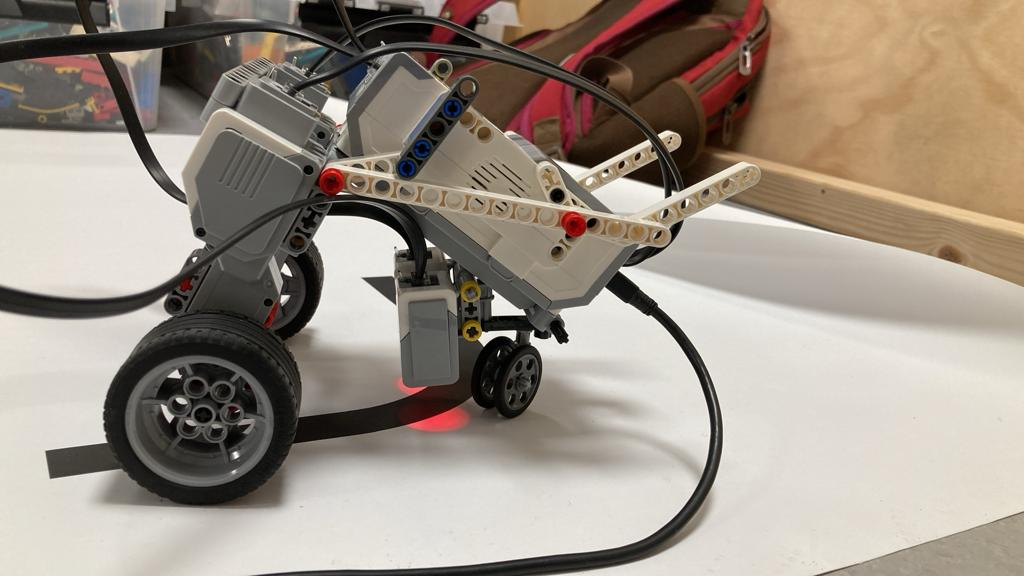
\includegraphics[width=\textwidth]{./figures/old-v-shape.jpeg}
		\caption{Original V shape design}
	\end{subfigure}

	\vspace{\baselineskip}

	\begin{subfigure}{0.4\textwidth}
		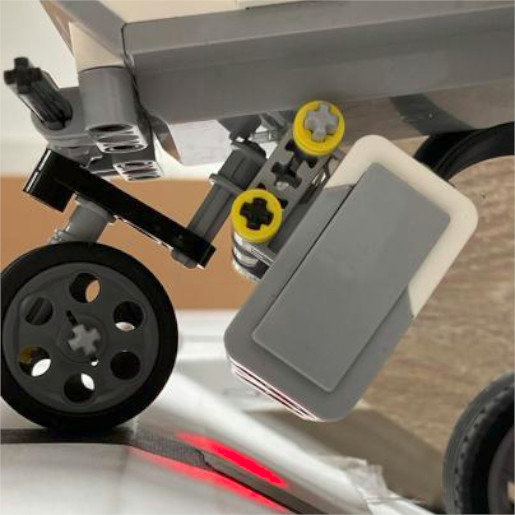
\includegraphics[width=\textwidth]{./figures/old-coaster-wheel.jpeg}
		\caption{Sensor placement detail}
	\end{subfigure}
	\hspace{0.01cm}
	\begin{subfigure}{0.4\textwidth}
		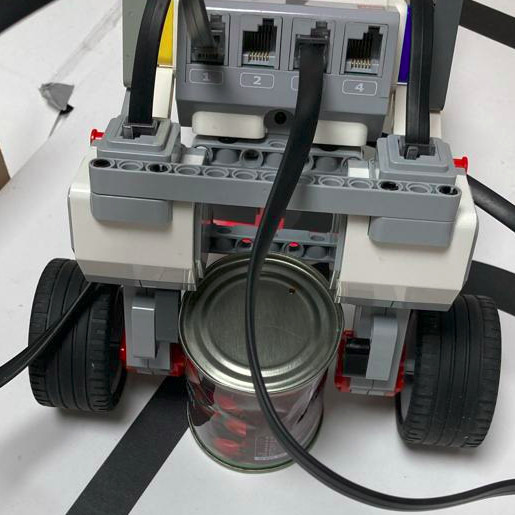
\includegraphics[width=\textwidth]{./figures/old-can-placement.jpeg}
		\caption{Convenient can area}
	\end{subfigure}

	\vspace{\baselineskip}

	\begin{subfigure}{0.8\textwidth}
		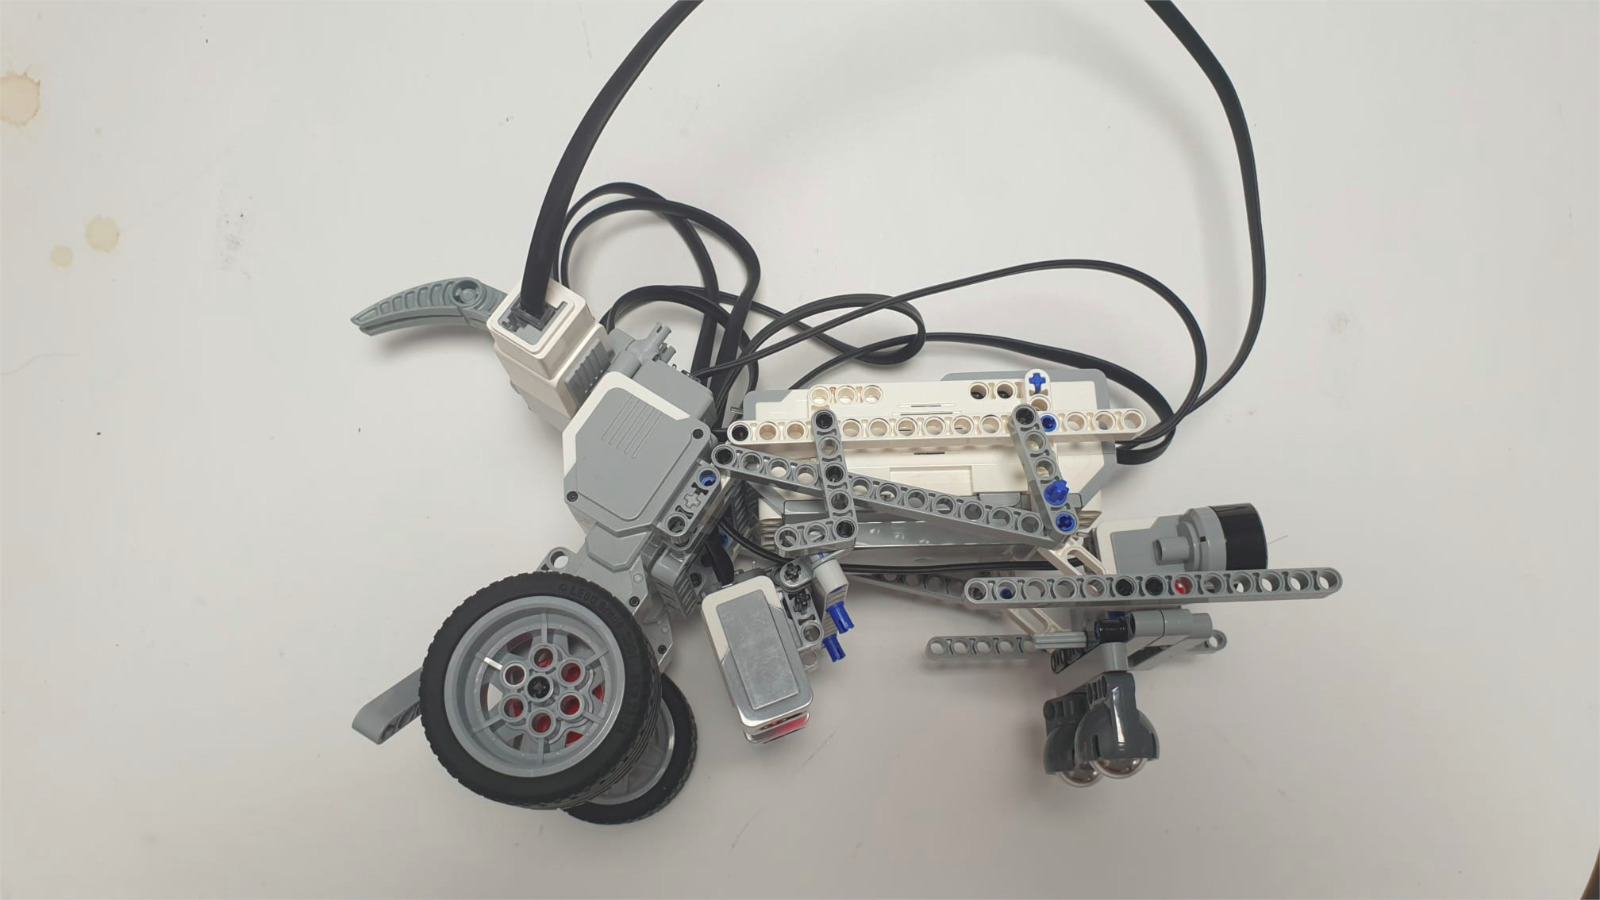
\includegraphics[width=\textwidth]{./figures/new-prototype.jpeg}
		\caption{Newest design iteration}
	\end{subfigure}

	\caption{Design changes with details}
	\label{fig:designChanges}

\end{figure}

\newpage

These factors led us to adapting a V shaped design that we kept through all the subsequent iterations. The design can
be seen in \ref{fig:designChanges}. This design, with motors and EVO brick forming a V, and with minimal added
structure elements, provided enough ground clearance to pass the slope edge and shifted weight to the front. When on
the slope, the brick side of the V shape became leveled, providing enough force for the wheels to grip.

Unfortunately, albeit providing improvement in many areas, the design also provided some unexpected challenges.
Because of the V shape, no surface was truly perpendicular to the ground, complicating the placement of line-following
sensors. The sensor placement itself went through multiple design iterations and was a major caveat of our design.
Our rigid body constraints didn't left much room for the sensor placement, resulting in only three possible
configurations -- between motors, below the V and in front of the vehicle.

We initially favoured the second variant mentioned, as it allowed for a convenient can capture mechanism in between
the motors \ref{fig:designChanges}. However, the sensors had to be placed rather high to prevent traversal issues, which
meant less response due to the distance from the surface. Unstable fixation of the sensors (see \ref{fig:designChanges})
led us to seek another minor redesign, that slightly changed the shape of the V and moved sensors to their final position
in the front of the vehicle.

\subsubsection*{Gripper}
\label{subsubsec:gripper}

Firstly, we tried to do a passive gripper, so that we would not need a third motor.The design included two claws. Where
one claw had a fixed position and the other claw was connected to a gear. The whole mechanism is visible
on~\ref{fig:gripper}.

\begin{figure}[!htbp]
	\centering
	\begin{subfigure}{0.4\textwidth}
		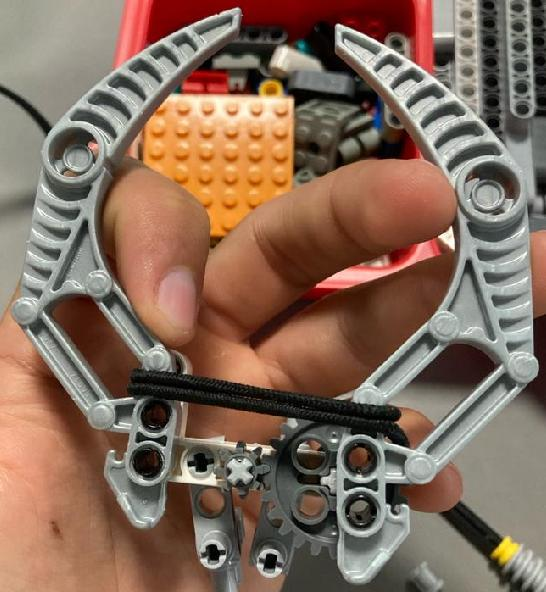
\includegraphics[width=\textwidth]{./figures/passiveGripper.jpeg}
		\caption{First implementation of a gripper as a passive gripper.}
		\label{fig:gripper}
	\end{subfigure}
	\hspace{0.01cm}
	\begin{subfigure}{0.4\textwidth}
		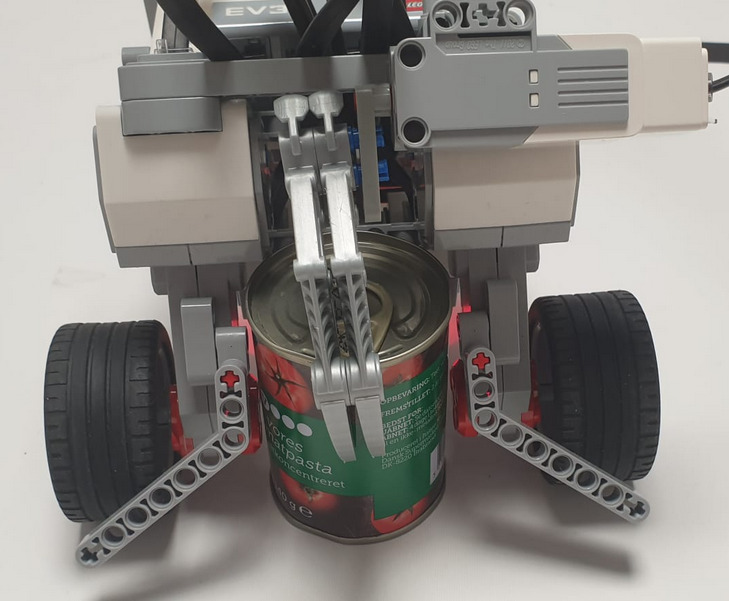
\includegraphics[width=\textwidth]{./figures/finalGripper.jpeg}
		\caption{Final version of the gripper}
		\label{fig:finalGripper}
	\end{subfigure}
\end{figure}

As we can see on the picture the grip was enforced by a rubber band. There was only one small issue with the gripper.
That was we needed a bit higher amount of force to activate it. The activation mechanism was as follows. The gripper was
stuck in opened state by a snail gear on a Lego crossed shape connector (visible in the bottom right corner
in~\ref{fig:gripper})

The claw was originally designed for a more generic 'cube' vehicle, but we kept the idea of a passive gripper even after
adapting the V shape. The space between motors, precisely fitting a knocked-down can, was not large enough to accommodate
a servo. However, the passive mechanism was hard to devise, and with our redesign which increased the space between
the motors we found the use of servo as an easier approach.

The servo also had one more promising advantage -- an ability to lift the can off the ground, thus shifting the balance.
We wanted to use this in our advantage and construct the mechanism so that the consequent weight shift backwards would
bring more weight to the rear of the vehicle, and the overall increase of weight near the wheel base would create
favourable conditions for the vehicle descent on the slope. This idea unfortunately was not implemented as we preferred
a more simple solution.

The final grabber was basically just a simple, servo operated latch, that closed on the can, securing it in standing
position between the motors, as can be seen in~\ref{fig:finalGripper}. As also visible from this picture, we also added
two bars covering the wheels that helped to lead the can in between the motors.

\subsubsection{Final design}
\label{subsubsec:final_design}

The final design brought many changes to the robot. We have kept the design directions from our previous design, but
we have changed the the way the motors were fixed to the brick. The new fixation provided more stiffness to the frame.
This meant the robot didn't need to be recalibrated after every transportation disassembly. It has also proven itself
to be easier for PID to control.

The final design also provided slightly more space between motors, which enabled us to fit in a servo with a claw-latch
mechanism, and also included a more favourable fixation of the ultrasound sensor in the front. The claw-latch mechanism
is made based on the behaviour of animals. When they want to keep the prey, kins or other stuff and not loose it, they
keep it in their claws. This approach is showed by the nature to be effective. Thus, we used it in our design.

Final design removed original coaster wheel design to accommodate for the change in angle. Instead, the device was
mounted with sled, as the sled was also more resilient to slope changes and impacts.

As the top of the slope still posed minor problems (slippery tape on the top resulted into oscillations and loss of
traction), we added a steel ball as a counterweight to the front of the vehicle to counter the problem.

For a more stable driving output, we have chosen the width between the optical sensors to be grater than the width of
the line. This measure brought nominal improvement to the driving capabilities, but it also meant, that being straight
on the line and not being on the line at all resulted in the same sensor output. This was the reason why we needed to
include an additional optical sensor placed between the ones already present, that was monitored by a function checking
for line presence, briefly described in \ref{subsubsec:can_localization}

\subsection{Control design}
\label{subsec:control_design}

\subsubsection{Approaches}
\label{subsubsec:approaches}

The first thing we have tried to do was to create a controller for line following. We have tried two approaches.
The first approach was to create a controller that will create a controller for left and right motor separately. In
that way we would have two controllers that will control the wheels based on the input from the sensors. The sensors
followed the \textit{Aggression principal} of \textit{Braintenberg vehicles}. The disadvantage that we had with this
approach was the presence of multiple PID control parameters. We had to set up the left and right wheel controller so
that their cooperation would be sufficient for line following.

The second approach was to create a \textit{differential drive}. For this we needed to have the distance between the
points of the wheels that touched the ground, radius of the wheels. For this approach we needed only one PID controller.
The difference with the previous approach is that the previous approach changes the speed of the motors and with that
it turns and the differential drive approach uses PID to change the turning rate where the forward speed is kept to be
the same.

All in all, we decided to go with the approach of \textit{differential drive} because of the reason, that it required
less parameters to set up. Every time we came to the laboratory we had to set up the parameters again and with every
modification of the mechanical structure (mentioned in \ref{subsec:mechanical_design}) we had to adjust the parameters.
That is why we decided to go with less parameters.

\subsubsection{Contol}
\label{subsubsec:control}

In our final implementation of the control of the robot we have finished with a schema that is displayed on
Fig.~\ref{fig:controlDiagram}.

\begin{figure}[hpbt!]
	\begin{center}
		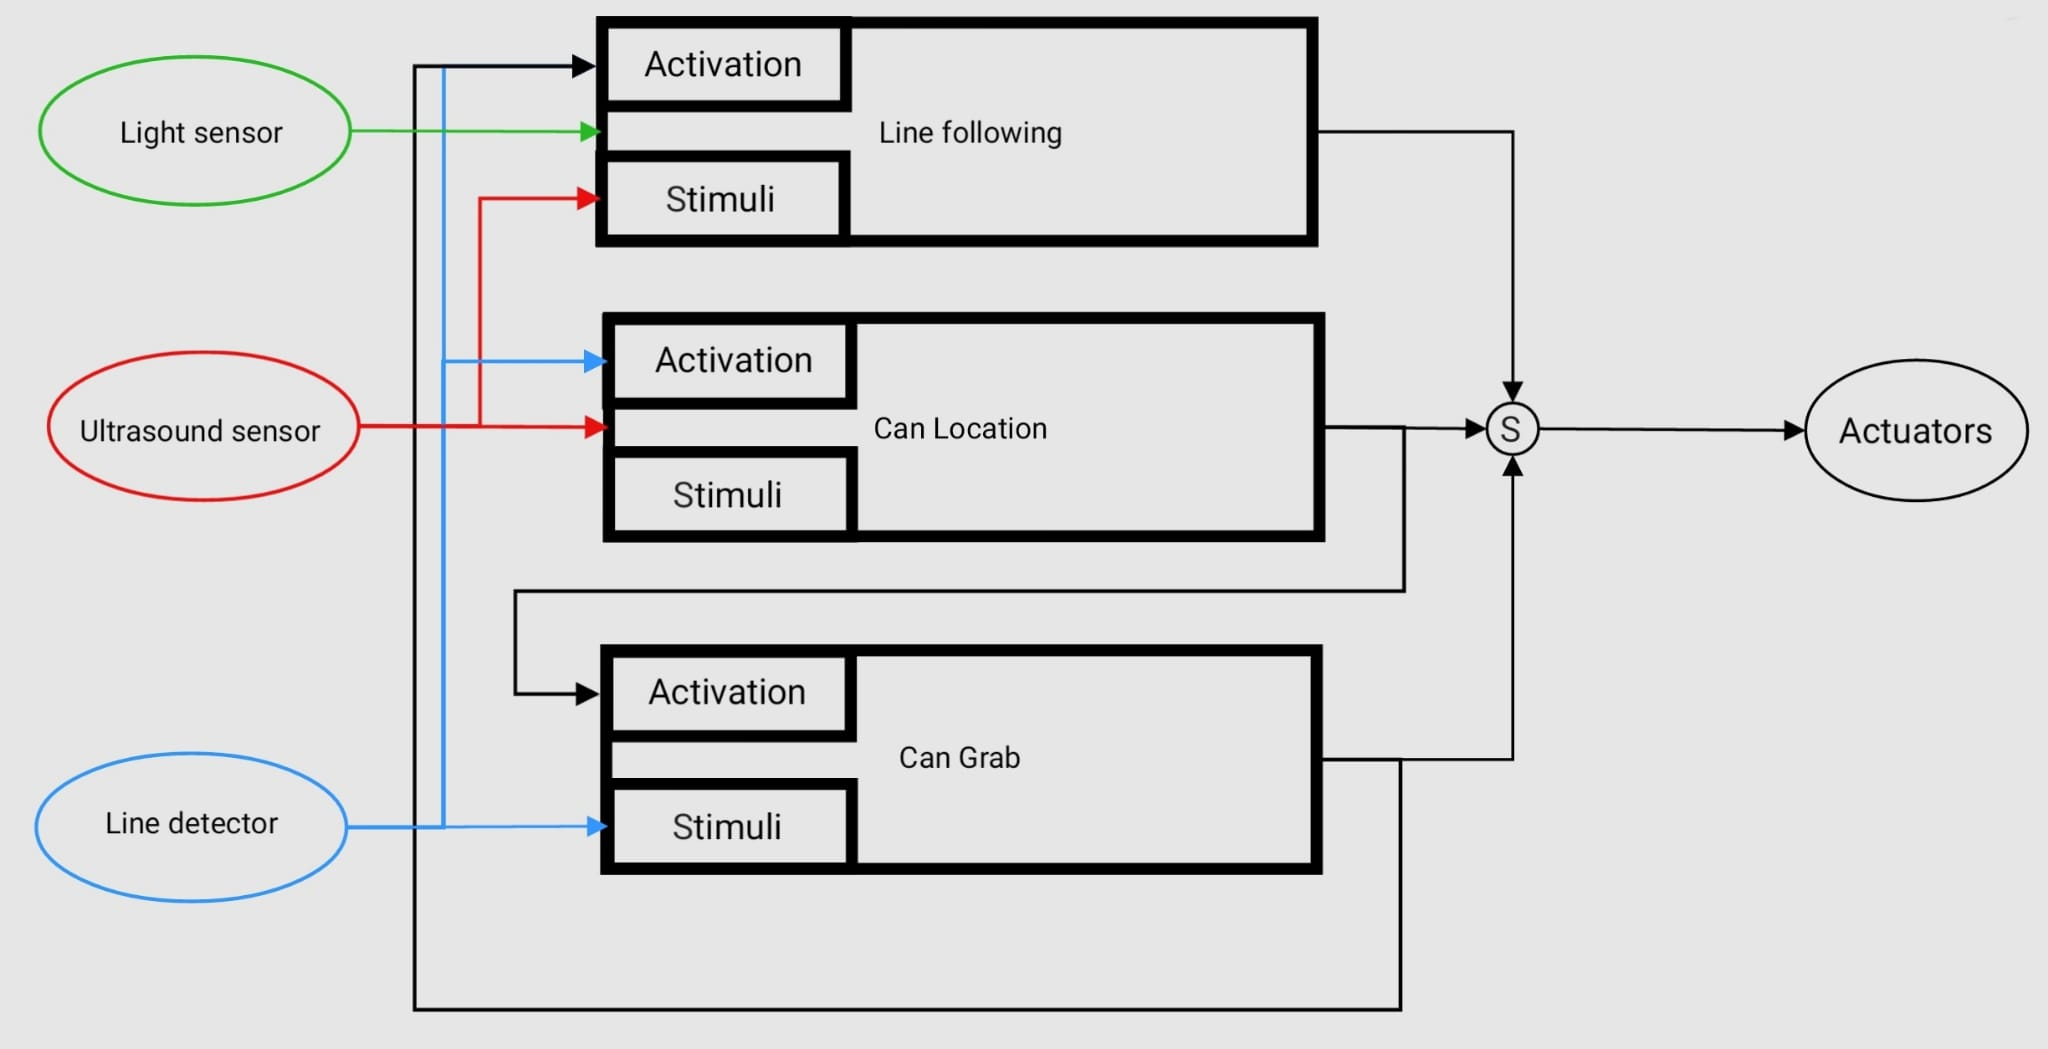
\includegraphics[width=0.95\textwidth]{"./figures/ControlDiagram.jpeg"}
	\end{center}
	\caption{The control diagram for the robot.}
	\label{fig:controlDiagram}
\end{figure}

We had three main behaviours:
\begin{itemize}
	\item Line following - behaviour that takes input from \textit{Light sensors} and uses it in PID controller.
	\item Can locating - behaviour that will take multiple values from the surrounding and based on the input
						 detects the can.
	\item Can grabbing - behaviour that based on the output of the localization goes and grabs the can.
\end{itemize}

We had three inputs from sensors:
\begin{itemize}
	\item Light sensors - sensors detecting, whether we are following the line correctly. We used reflection function
		  to get the input from both of them,
	\item Ultrasound sensor - sensor that is scanning the change of distances in front of the robot, so that we can
		  detect the can,
	\item Line detector (colour sensor) - sensor used for end of line detection. This sensor was used as an activation
		  function for jumping between the sates of \textit{Line following} and \textit{Can location}.
\end{itemize}

The output\textit{Actuators} is meant to be the left and right motor and the gripper. The state we are currently in takes
full control of all the motors at the same time.

The line following is activated either by \textit{Line detector} when it finds a line or by the finished operation
of \textit{Can grabbing}. It is stimulated by the ultrasound detection. This signal at the same time is used as an
input to the \textit{Can localization} behaviour. This behaviour is activated by loosing the line. In this behaviour
we make an initial turn to the left and we scan the distance from the robot from the ultrasound sensor. This we store
in memory and do a first derivation of the measured data. We knew that the can will be located at least 10 cm from the
wall, that is why we tried to detect the change of more then 10 cm. This approach was a bit troublesome on the lower
platform where there was no wall, so we limited the difference by 25 cm. The last state \textit{Can grabbing} is
activated by the output of the \textit{Can localization}, here if we found the can we turned around and grabbed the can
with the gripper as mentioned in~\ref{subsubsec:final_design}.

\subsubsection{PID controller}
\label{subsubsec:pid}

As mentioned before in~\ref{subsubsec:approaches}, we ended up using the \textit{differential drive}. The final design
of the robot had the distance between points of the wheels that touch the ground \textit{142 mm} apart. The wheel
diameter was \textit{40 cm}. Our forward speed changed over time.

With the pid controller we tried two approaches. The first one was a typical PID controller and the second one is
an IP controller.

Firstly, we started with speed of \textit{100 mm/s} and the parameters for PID controller were respectively \textit{1},
\textit{0}, \textit{0}. After we saw how the robot behaves with this basic PID controller we could adjust the coefficients
even more. When we saw that the line following algorithm is starting to oscillate with only \textit{proportional}
coefficient we lowered the proportional part and we started increasing the \textit{integral} coefficient.

When we had the sled in the front of the robot the proportional part could go up to 80 or even 90 due to the friction of
the sled. When we removed it the proportional part stabilized at around 20 to 23. In the end we ended up with
proportional coefficient with value of \textit{21}.

The \textit{integral} part was a bit tricky, we had to be more precise with this one because even a small change of
\textit{0.01} made the whole system unstable. Finally, after multiple experiments we ended up the value of \textit{0.075}.

We also tried to use the derivative part, however this approach was not successful and even though we could stabilize
the system on straight line we were not able to make the turns that required for the robot to turn while seeing the line
only partially.

The second approach, using the IP controller, was tried because of the reason that the IP controller is known to be more
stabilizing. This approach showed up to be actually worse than the PID controller. Thus, we continued with the PID
controller.

\subsubsection{Can localization}
\label{subsubsec:can_localization}

Can localization was done using a third \textit{colour sensor}. This sensor was measuring the reflection from the surface
between the other two colour sensors. If a small reflection was detected that meant that we are on the line. However,
higher reflection meant that we lost the line. The detection of end of the line was done the following way.

The colour sensor was checking for the line. If the line was lost the internal counting was initiated, if we did not
detect a line under the robot multiple times we initiated Can localization behaviour.

Firstly, we turned 65\textdegree to the left. After achieving this rotation we started doing small turns to
the right. After every small turn we checked for an object in front of the robot. This way we got 42 measurements. Then
we calculated the gradient of this function. If a change higher than 100 mm but lower than 250 mm was detected, that
meant, that we found the can.

The scan and the consecutive gradient, were done only in one direction, for sake of simplicity. With a short
addition, a second scan could be added in the opposite direction, leading to a more precise position calculation.

\subsubsection*{Can grabbing}
\label{subsubsec:can-grabbing}

After detecting the position of the can, the robot was programmed to turn around 180\textdegree and reverse back into
the can. We knew the distance of the robot to the can and we used that to get to our goal. We have tested the scenario
many times to set correct constants to the behavior. After that, the latch would be rotated into a set position,
enclosing the can between optical line sensors and motors.

\section{Evaluation methods and results}
\label{sec:evaluation_methods_and_results}

In the preliminary report we mentioned multiple testing methods:

\begin{enumerate}
	\item Line following test,
	\item Ability to climb the ramp,
	\item Grabbing mechanism,
	\item Time measuring to complete the race.
\end{enumerate}

The line following was tested every time we arrived to the laboratory. The first test was always done on a straight line
with a small turn. This map we found in the laboratory and was available to all the students. When that test passed, we
tried the line following algorithm on the bottom floor. Solving a more simple map first meant we achieved a
\textit{generaly good} control before fine tuning the response on a more complicated one. This approach to the test was
always successful.

The whole robot design was created with the thought, that it should be able to climb the ramp. That was the first thing
that we tested. It did not matter what design we created, the ramp climbing ability was the top priority for us. The
second priority was the PID coefficient efficiency for the line following algorithm.

We thought about the gripper mechanism multiple times. As we mentioned in the final report: \textit{"That may not be the
best solution, so we will test the gripper and if we find out that it is not possible to grab the can, we will change our
approach.The robot's performance will be measured by time.  We will measure the time it takes to complete the task and
we will try to optimise it."} It actually was not the best solution. Thus, we chose to use an active gripper.
We tested the gripper on the top floor and also on the ramp. While not on the ramp the claws were sufficient enough to
keep the can inside the cavity. When we got to the ramp we had issues with keeping the can in the gripper and with the
wheel grip.

Unfortunately, we could not complete the runs all the time. We had issues with the gripper, the traction while going
down the ramp and sometimes with line following. With a help on the ramp (to avoid a slip) we were able to retrieve the
can several times, however the underlying problems would be hard to fix without a major change of concept.

\newpage

\section{Discussion and conclusions}
\label{sec:discussion_and_conclusions}

What we thought about changing in the implementation of the robot was changing the robot's structure from the beginning.
One of the changes discussed was opting for a four wheel drive vehicle, which would provide for a better traction with
nearly the same weight and the same motor count. The wheels would be connected with gears so that we could mechanically
influence the torque. Additionally, a wider four wheel platform closer to the ground would provide a better sensor placement
in the middle of the vehicle. The sensors could also be closer to the ground without running into traversal issues.
Moreover, the robot would create a shadow enclosing the sensors. Thus, we could have better sensor readings.

A different platform could also enable us to create a more useful grabbing mechanism, hopefully helping us climbing
down the ramp without loosing the can as discussed in previous section.

All in all, we created an implementation of the mobile robot so that it could follow the line, climb up the ramp and
grab the can. The implementation was successful in avoiding some of the challenges we identified in the preliminary
report, although it was not able to complete the rescue mission in its entirety.

\end{document}

